\section{Basisproblemet}
Vi har indgået en kontrakt med ejeren af et gaslager, hvori der kan lagres naturgas. Vi har lejet dette gaslager for et år, og vi skal nu forsøge at maksimere profitten ved køb og salg af gassen. Vi har en forward-kurve på prisen, således at vi til hver en tid i lejekontrakten kan se hvad prisen for gas bliver. Der er øvre og nedre grænser for beholdningen i gaslaget, og ved lejekontraktens udløb vil ejeren købe den resterende gas til prisen på det tidspunkt. Vi opstillere en tabel \ref{table:1} med de forskellige variable, som vi skal bruge til at løse optimeringsproblemet:

\begin{table}[h!]
\centering
\begin{tabular}{||c | c||} 
 \hline
 Variabel & Beskrivelse \\ [0.5ex] 
 \hline\hline
 $t$ & Tidsskridt  \\ 
 $T$ & Sluttid  \\
 $q_{t}$ & Gasenheder til tiden $t$  \\
 $\Delta q_{t}$ & Ændringen i gasenheder,    $q_{t}-q_{t-1}$ \\
 $q_{0}$ & Gasenheder i starten af lejeperioden  \\
 $q_{min}$ & Den nedre grænse for gasenheder \\ 
 $q_{max}$ & Den øvre grænse for gasenheder \\
 $u_{max}$ & Antal gasenheder der kan tages ud af lageret mellem to tidsskridt \\ 
 $i_{max}$ & Antal gasenheder der kan sættes ind på lageret mellem to tidsskridt \\ 
 $p_{t}$ & En forward pris i Euro på en gasenhed  \\
 $r$ & En fast årlig diskonteringsrente  \\
 [1ex] 
 \hline
\end{tabular}
\caption{Table to test captions and labels}
\label{table:1}
\end{table}

I basisproblemet er $q_{min}$, $q_{max}$, $i_{max}$ og $u_{max}$ statiske. Det vil sige, at de ikke ændrer sig i hele lejeperiden. Hvis vi ønsker at maksimere nutidsværdien af profitten fås:
\begin{equation}
\max_{\Delta p_{t}} \Bigg\{ -\sum_{t=1}^{T} \mathrm{e}^{-r\frac{t}{T}} \Delta q_{t} p_{t}+ \mathrm{e}^{-r}q_{T}p_{T} \Bigg\} \
\end{equation}
Her ville bibetingelserne være:\\
1. $q_{min} \leq q_{t} \leq q_{max}$\\
2. $\Delta q_{t} \in \{-u_{max},-u_{max}+1,\cdots,-1,0,1,\cdots,i_{max}-1,i_{max} \}$ \\
for $t \in \{1,\cdots,T\}$ hvor gasmængden lagret til tiden, $t$, er $q_{t}=q_{0}+\sum_{s=1}^{t} \Delta q_{s}$.

\section{Grafen for basisproblemet}
Vi kan med udgangspunkt i afsnittet om grafteori opstille en graf for vores basisproblem. Grafen er en simpel, orienteret, vægtet graf. Vi opstiller et simplificeret eksempel på grafen med følgende data:
\begin{itemize}
  \item $t \in \{1,2,3,4,5,6\}$
  \item $q_{0}=1$
  \item $q_{min}=0$
  \item $q_{max}=2$
  \item $i_{max}=1$
  \item $u_{max}=1$
  \item $p_{6}=(20,22,25,18,15,15)$
\end{itemize}

\begin{figure}[H]
\centering
	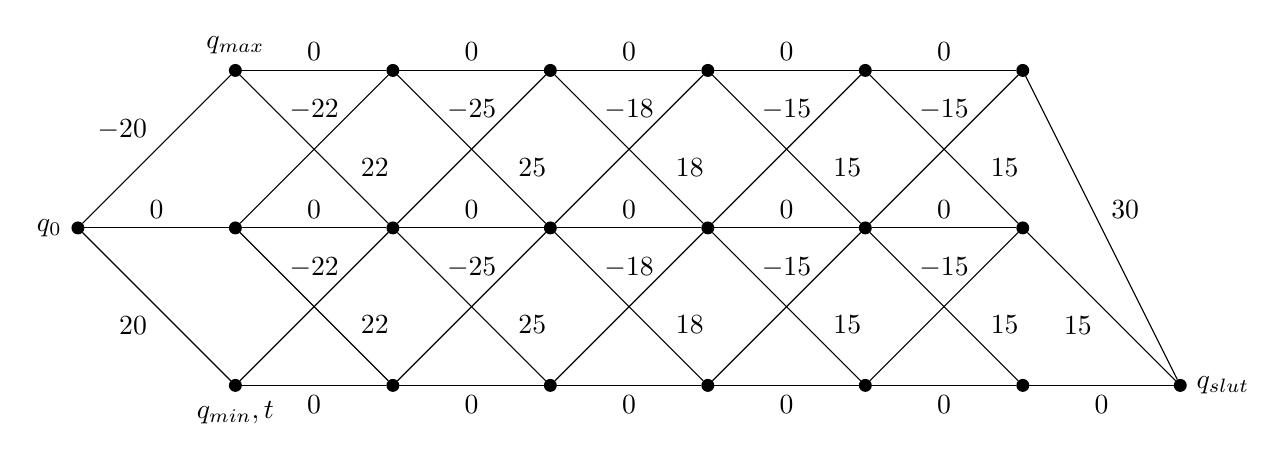
\begin{tikzpicture}

      \tikzset{enclosed/.style={draw, circle, inner sep=0pt, minimum size=.15cm, fill=black}}
%% Vertices
      	\node[enclosed, label={left: $q_{0}$}] (v1) at (0,2) {};
      	\node[enclosed, label={below: $q_{min},   t$}] (v2) at (2,0) {};
    		\node[enclosed, label={below: }] (v3) at (2,2) {};
  	    \node[enclosed, label={above: $q_{max}$}] (v4) at (2,4) {};
     	\node[enclosed, label={left: }] (v5) at (4,0) {};
     	\node[enclosed, label={left: }] (v6) at (4,2) {};
     	\node[enclosed, label={left: }] (v7) at (4,4) {};
     	\node[enclosed, label={right: }] (v8) at (6,0) {};
     	\node[enclosed, label={right: }] (v9) at (6,2) {};
     	\node[enclosed, label={right: }] (v10) at (6,4) {};
     	\node[enclosed, label={right: }] (v11) at (8,0) {};
     	\node[enclosed, label={below: }] (v12) at (8,2) {};
      	\node[enclosed, label={below: }] (v13) at (8,4) {};
  	    \node[enclosed, label={below: }] (v14) at (10,0) {};
  	    \node[enclosed, label={below: }] (v15) at (10,2) {};
     	\node[enclosed, label={below: }] (v16) at (10,4) {};
     	\node[enclosed, label={below: }] (v17) at (12,0) {};
     	 \node[enclosed, label={below:}] (v18) at (12,2) {};
     	\node[enclosed, label={below: }] (v19) at (12,4) {};
     	\node[enclosed, label={right: $q_{slut}$ }] (v20) at (14,0) {};
     	
%Edges
		\path (v1) edge node[midway, sloped, above, label={below: $20$ }] {} (v2);
		\path (v1) edge node[midway, sloped, below, label={above: $0$ }] {} (v3);
		\path (v1) edge node[midway, sloped, below, label={above: $-20$ }] {} (v4);
		\path (v2) edge node[midway, sloped, above, label={below: $0$ }] {} (v5);
		\path (v2) edge node[midway, above, label={above: $-22$ }] {} (v6);
		\path (v3) edge node[near end, sloped, below, label={above: $22$ }] {} (v5);
		\path (v3) edge node[midway, sloped, below, label={above: $0$ }] {} (v6);
		\path (v3) edge node[midway, above, label={above: $-22$ }] {} (v7);
		\path (v4) edge node[near end, sloped, below, label={above: $22$ }] {} (v6);
		\path (v4) edge node[midway, sloped, below, label={above: $0$ }] {} (v7);
		\path (v5) edge node[midway, sloped, above, label={below: $0$ }] {} (v8);
		\path (v5) edge node[midway, above, label={above: $-25$ }] {} (v9);
		\path (v6) edge node[near end, sloped, below, label={above: $25$ }] {} (v8);
		\path (v6) edge node[midway, sloped, below, label={above: $0$ }] {} (v9);
		\path (v6) edge node[midway, above, label={above: $-25$ }] {} (v10);
		\path (v7) edge node[near end, sloped, below, label={above: $25$ }] {} (v9);
		\path (v7) edge node[midway, sloped, below, label={above: $0$ }] {} (v10);
		\path (v8) edge node[midway, sloped, above, label={below: $0$ }] {} (v11);
		\path (v8) edge node[midway, above, label={above: $-18$ }] {} (v12);
		\path (v9) edge node[near end, sloped, below, label={above: $18$ }] {} (v11);
		\path (v9) edge node[midway, sloped, below, label={above: $0$ }] {} (v12);
		\path (v9) edge node[midway, above, label={above: $-18$ }] {} (v13);
		\path (v10) edge node[near end, sloped, below, label={above: $18$ }] {} (v12);
		\path (v10) edge node[midway, sloped, below, label={above: $0$ }] {} (v13);
		\path (v11) edge node[midway, sloped, above, label={below: $0$ }] {} (v14);
		\path (v11) edge node[midway, above, label={above: $-15$ }] {} (v15);
		\path (v12) edge node[near end, sloped, below, label={above: $15$ }] {} (v14);
		\path (v12) edge node[midway, sloped, below, label={above: $0$ }] {} (v15);
		\path (v12) edge node[midway, above, label={above: $-15$ }] {} (v16);
		\path (v13) edge node[near end, sloped, below, label={above: $15$ }] {} (v15);
		\path (v13) edge node[midway, sloped, below, label={above: $0$ }] {} (v16);
		\path (v14) edge node[midway, sloped, above, label={below: $0$ }] {} (v17);
		\path (v14) edge node[midway, above, label={above: $-15$ }] {} (v18);
		\path (v15) edge node[near end, sloped, below, label={above: $15$ }] {} (v17);
		\path (v15) edge node[midway, sloped, below, label={above: $0$ }] {} (v18);
		\path (v15) edge node[midway, above, label={above: $-15$ }] {} (v19);
		\path (v16) edge node[near end, sloped, below, label={above: $15$ }] {} (v18);
		\path (v16) edge node[midway, sloped, below, label={above: $0$ }] {} (v19);
		\path (v17) edge node[midway, sloped, above, label={below: $0$ }] {} (v20);
		\path (v18) edge node[midway, sloped, above, label={below: $15$ }] {} (v20);
		\path (v19) edge node[midway, sloped, below, label={above: $30$ }] {} (v20);
	\end{tikzpicture}
	\caption{Graf for forsimplet gaslager.}
	\label{fig.gaslager_graf}
\end{figure}

Vi ganger med -1 for at gøre det til et korteste vej problem:

\begin{figure}[H]
\centering
	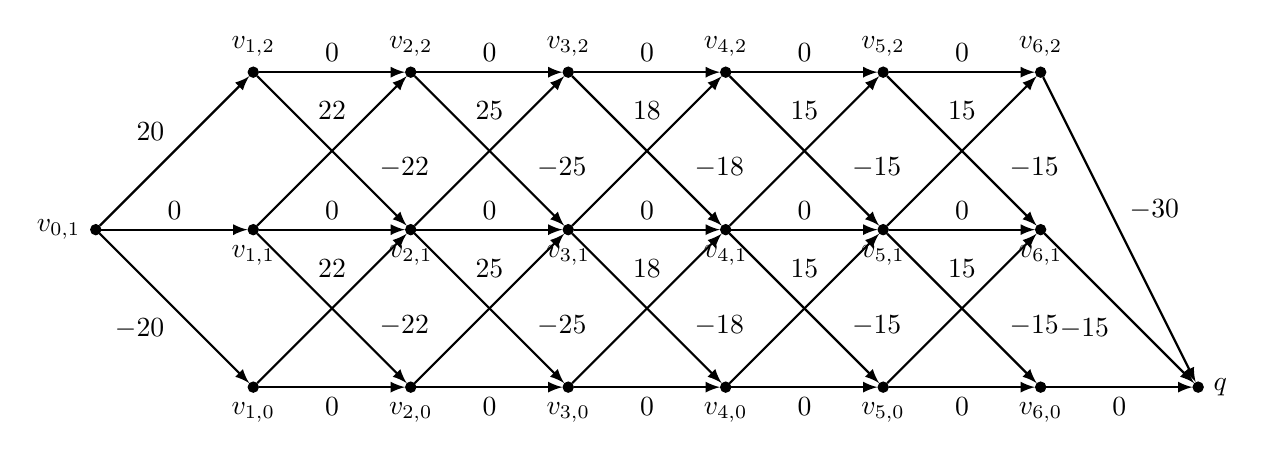
\begin{tikzpicture}

       \tikzset{enclosed/.style={draw, circle, inner sep=0pt, minimum size=.13cm, fill=black}}
%% Vertices
      	\node[enclosed, label={left: $v_{0,1}$}] (v1) at (0,2) {};
      	\node[enclosed, label={below: $v_{1,0}$}] (v2) at (2,0) {};
    		\node[enclosed, label={below: $v_{1,1}$}] (v3) at (2,2) {};
  	    \node[enclosed, label={above: $v_{1,2}$}] (v4) at (2,4) {};
     	\node[enclosed, label={below: $v_{2,0}$}] (v5) at (4,0) {};
     	\node[enclosed, label={below: $v_{2,1}$ }] (v6) at (4,2) {};
     	\node[enclosed, label={above: $v_{2,2}$}] (v7) at (4,4) {};
     	\node[enclosed, label={below:$v_{3,0}$ }] (v8) at (6,0) {};
     	\node[enclosed, label={below:$v_{3,1}$ }] (v9) at (6,2) {};
     	\node[enclosed, label={above:$v_{3,2}$ }] (v10) at (6,4) {};
     	\node[enclosed, label={below: $v_{4,0}$ }] (v11) at (8,0) {};
     	\node[enclosed, label={below:$v_{4,1}$ }] (v12) at (8,2) {};
      	\node[enclosed, label={above:$v_{4,2}$ }] (v13) at (8,4) {};
  	    \node[enclosed, label={below: $v_{5,0}$}] (v14) at (10,0) {};
  	    \node[enclosed, label={below:$v_{5,1}$ }] (v15) at (10,2) {};
     	\node[enclosed, label={above: $v_{5,2}$ }] (v16) at (10,4) {};
     	\node[enclosed, label={below:$v_{6,0}$ }] (v17) at (12,0) {};
     	 \node[enclosed, label={below:$v_{6,1}$}] (v18) at (12,2) {};
     	\node[enclosed, label={above: $v_{6,2}$}] (v19) at (12,4) {};
     	\node[enclosed, label={right: $q_{\slut}$ }] (v20) at (14,0) {};
     	
%Edges
		\path[->,>=latex,thick] (v1) edge node[midway, sloped, above, label={below: $-20$ }] {} (v2);
		\path[->,>=latex,thick] (v1) edge node[midway, sloped, below, label={above: $0$ }] {} (v3);
		\path[->,>=latex,thick] (v1) edge node[midway, sloped, below, label={above: $20$ }] {} (v4);
		\path[->,>=latex,thick] (v2) edge node[midway, sloped, above, label={below: $0$ }] {} (v5);
		\path[->,>=latex,thick] (v2) edge node[midway, above, label={above: $22$ }] {} (v6);
		\path[->,>=latex,thick] (v3) edge node[near end, sloped, below, label={above: $-22$ }] {} (v5);
		\path[->,>=latex,thick] (v3) edge node[midway, sloped, below, label={above: $0$ }] {} (v6);
		\path[->,>=latex,thick] (v3) edge node[midway, above, label={above: $22$ }] {} (v7);
		\path[->,>=latex,thick] (v4) edge node[near end, sloped, below, label={above: $-22$ }] {} (v6);
		\path[->,>=latex,thick] (v4) edge node[midway, sloped, below, label={above: $0$ }] {} (v7);
		\path[->,>=latex,thick] (v5) edge node[midway, sloped, above, label={below: $0$ }] {} (v8);
		\path[->,>=latex,thick] (v5) edge node[midway, above, label={above: $25$ }] {} (v9);
		\path[->,>=latex,thick] (v6) edge node[near end, sloped, below, label={above: $-25$ }] {} (v8);
		\path[->,>=latex,thick] (v6) edge node[midway, sloped, below, label={above: $0$ }] {} (v9);
		\path[->,>=latex,thick] (v6) edge node[midway, above, label={above: $25$ }] {} (v10);
		\path[->,>=latex,thick] (v7) edge node[near end, sloped, below, label={above: $-25$ }] {} (v9);
		\path[->,>=latex,thick] (v7) edge node[midway, sloped, below, label={above: $0$ }] {} (v10);
		\path[->,>=latex,thick] (v8) edge node[midway, sloped, above, label={below: $0$ }] {} (v11);
		\path[->,>=latex,thick] (v8) edge node[midway, above, label={above: $18$ }] {} (v12);
		\path[->,>=latex,thick] (v9) edge node[near end, sloped, below, label={above: $-18$ }] {} (v11);
		\path[->,>=latex,thick] (v9) edge node[midway, sloped, below, label={above: $0$ }] {} (v12);
		\path[->,>=latex,thick] (v9) edge node[midway, above, label={above: $18$ }] {} (v13);
		\path[->,>=latex,thick] (v10) edge node[near end, sloped, below, label={above: $-18$ }] {} (v12);
		\path[->,>=latex,thick] (v10) edge node[midway, sloped, below, label={above: $0$ }] {} (v13);
		\path[->,>=latex,thick] (v11) edge node[midway, sloped, above, label={below: $0$ }] {} (v14);
		\path[->,>=latex,thick] (v11) edge node[midway, above, label={above: $15$ }] {} (v15);
		\path[->,>=latex,thick] (v12) edge node[near end, sloped, below, label={above: $-15$ }] {} (v14);
		\path[->,>=latex,thick] (v12) edge node[midway, sloped, below, label={above: $0$ }] {} (v15);
		\path[->,>=latex,thick] (v12) edge node[midway, above, label={above: $15$ }] {} (v16);
		\path[->,>=latex,thick] (v13) edge node[near end, sloped, below, label={above: $-15$ }] {} (v15);
		\path[->,>=latex,thick] (v13) edge node[midway, sloped, below, label={above: $0$ }] {} (v16);
		\path[->,>=latex,thick] (v14) edge node[midway, sloped, above, label={below: $0$ }] {} (v17);
		\path[->,>=latex,thick] (v14) edge node[midway, above, label={above: $15$ }] {} (v18);
		\path[->,>=latex,thick] (v15) edge node[near end, sloped, below, label={above: $-15$ }] {} (v17);
		\path[->,>=latex,thick] (v15) edge node[midway, sloped, below, label={above: $0$ }] {} (v18);
		\path[->,>=latex,thick] (v15) edge node[midway, above, label={above: $15$ }] {} (v19);
		\path[->,>=latex,thick] (v16) edge node[near end, sloped, below, label={above: $-15$ }] {} (v18);
		\path[->,>=latex,thick] (v16) edge node[midway, sloped, below, label={above: $0$ }] {} (v19);
		\path[->,>=latex,thick] (v17) edge node[midway, sloped, above, label={below: $0$ }] {} (v20);
		\path[->,>=latex,thick] (v18) edge node[midway, sloped, above, label={below: $-15$ }] {} (v20);
		\path[->,>=latex,thick] (v19) edge node[midway, sloped, below, label={above: $-30$ }] {} (v20);
	\end{tikzpicture}
	\caption{Graf for forsimplet gaslager ganget med -1.}
	\label{fig.gaslager_graf}
\end{figure}

Vi lægger 30 til alle tal, da Dijkstras algoritme kun virker på ikke-negative tal:


\begin{figure}[H]
\centering
	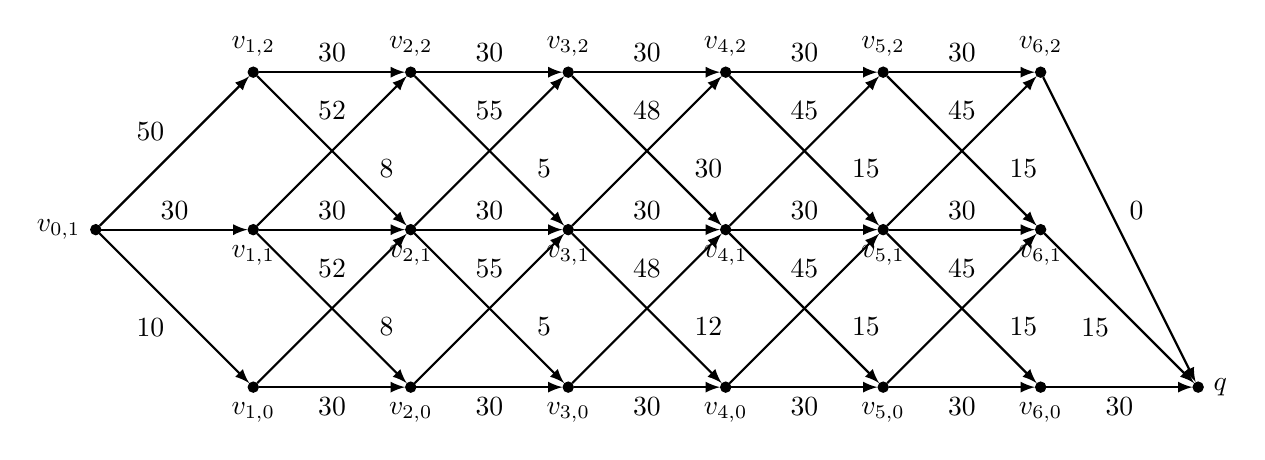
\begin{tikzpicture}

       \tikzset{enclosed/.style={draw, circle, inner sep=0pt, minimum size=.13cm, fill=black}}
%% Vertices
      	\node[enclosed, label={left: $v_{0,1}$}] (v1) at (0,2) {};
      	\node[enclosed, label={below: $v_{1,0}$}] (v2) at (2,0) {};
    		\node[enclosed, label={below: $v_{1,1}$}] (v3) at (2,2) {};
  	    \node[enclosed, label={above: $v_{1,2}$}] (v4) at (2,4) {};
     	\node[enclosed, label={below: $v_{2,0}$}] (v5) at (4,0) {};
     	\node[enclosed, label={below: $v_{2,1}$ }] (v6) at (4,2) {};
     	\node[enclosed, label={above: $v_{2,2}$}] (v7) at (4,4) {};
     	\node[enclosed, label={below:$v_{3,0}$ }] (v8) at (6,0) {};
     	\node[enclosed, label={below:$v_{3,1}$ }] (v9) at (6,2) {};
     	\node[enclosed, label={above:$v_{3,2}$ }] (v10) at (6,4) {};
     	\node[enclosed, label={below: $v_{4,0}$ }] (v11) at (8,0) {};
     	\node[enclosed, label={below:$v_{4,1}$ }] (v12) at (8,2) {};
      	\node[enclosed, label={above:$v_{4,2}$ }] (v13) at (8,4) {};
  	    \node[enclosed, label={below: $v_{5,0}$}] (v14) at (10,0) {};
  	    \node[enclosed, label={below:$v_{5,1}$ }] (v15) at (10,2) {};
     	\node[enclosed, label={above: $v_{5,2}$ }] (v16) at (10,4) {};
     	\node[enclosed, label={below:$v_{6,0}$ }] (v17) at (12,0) {};
     	 \node[enclosed, label={below:$v_{6,1}$}] (v18) at (12,2) {};
     	\node[enclosed, label={above: $v_{6,2}$}] (v19) at (12,4) {};
     	\node[enclosed, label={right: $q_{\slut}$ }] (v20) at (14,0) {};
     	
%Edges
		\path[->,>=latex,thick] (v1) edge node[midway, sloped, above, label={below: $10$ }] {} (v2);
		\path[->,>=latex,thick] (v1) edge node[midway, sloped, below, label={above: $30$ }] {} (v3);
		\path[->,>=latex,thick] (v1) edge node[midway, sloped, below, label={above: $50$ }] {} (v4);
		\path[->,>=latex,thick] (v2) edge node[midway, sloped, above, label={below: $30$ }] {} (v5);
		\path[->,>=latex,thick] (v2) edge node[midway, above, label={above: $52$ }] {} (v6);
		\path[->,>=latex,thick] (v3) edge node[near end, sloped, below, label={above: $8$ }] {} (v5);
		\path[->,>=latex,thick] (v3) edge node[midway, sloped, below, label={above: $30$ }] {} (v6);
		\path[->,>=latex,thick] (v3) edge node[midway, above, label={above: $52$ }] {} (v7);
		\path[->,>=latex,thick] (v4) edge node[near end, sloped, below, label={above: $8$ }] {} (v6);
		\path[->,>=latex,thick] (v4) edge node[midway, sloped, below, label={above: $30$ }] {} (v7);
		\path[->,>=latex,thick] (v5) edge node[midway, sloped, above, label={below: $30$ }] {} (v8);
		\path[->,>=latex,thick] (v5) edge node[midway, above, label={above: $55$ }] {} (v9);
		\path[->,>=latex,thick] (v6) edge node[near end, sloped, below, label={above: $5$ }] {} (v8);
		\path[->,>=latex,thick] (v6) edge node[midway, sloped, below, label={above: $30$ }] {} (v9);
		\path[->,>=latex,thick] (v6) edge node[midway, above, label={above: $55$ }] {} (v10);
		\path[->,>=latex,thick] (v7) edge node[near end, sloped, below, label={above: $5$ }] {} (v9);
		\path[->,>=latex,thick] (v7) edge node[midway, sloped, below, label={above: $30$ }] {} (v10);
		\path[->,>=latex,thick] (v8) edge node[midway, sloped, above, label={below: $30$ }] {} (v11);
		\path[->,>=latex,thick] (v8) edge node[midway, above, label={above: $48$ }] {} (v12);
		\path[->,>=latex,thick] (v9) edge node[near end, sloped, below, label={above: $12$ }] {} (v11);
		\path[->,>=latex,thick] (v9) edge node[midway, sloped, below, label={above: $30$ }] {} (v12);
		\path[->,>=latex,thick] (v9) edge node[midway, above, label={above: $48$ }] {} (v13);
		\path[->,>=latex,thick] (v10) edge node[near end, sloped, below, label={above: $30$ }] {} (v12);
		\path[->,>=latex,thick] (v10) edge node[midway, sloped, below, label={above: $30$ }] {} (v13);
		\path[->,>=latex,thick] (v11) edge node[midway, sloped, above, label={below: $30$ }] {} (v14);
		\path[->,>=latex,thick] (v11) edge node[midway, above, label={above: $45$ }] {} (v15);
		\path[->,>=latex,thick] (v12) edge node[near end, sloped, below, label={above: $15$ }] {} (v14);
		\path[->,>=latex,thick] (v12) edge node[midway, sloped, below, label={above: $30$ }] {} (v15);
		\path[->,>=latex,thick] (v12) edge node[midway, above, label={above: $45$ }] {} (v16);
		\path[->,>=latex,thick] (v13) edge node[near end, sloped, below, label={above: $15$ }] {} (v15);
		\path[->,>=latex,thick] (v13) edge node[midway, sloped, below, label={above: $30$ }] {} (v16);
		\path[->,>=latex,thick] (v14) edge node[midway, sloped, above, label={below: $30$ }] {} (v17);
		\path[->,>=latex,thick] (v14) edge node[midway, above, label={above: $45$ }] {} (v18);
		\path[->,>=latex,thick] (v15) edge node[near end, sloped, below, label={above: $15$ }] {} (v17);
		\path[->,>=latex,thick] (v15) edge node[midway, sloped, below, label={above: $30$ }] {} (v18);
		\path[->,>=latex,thick] (v15) edge node[midway, above, label={above: $45$ }] {} (v19);
		\path[->,>=latex,thick] (v16) edge node[near end, sloped, below, label={above: $15$ }] {} (v18);
		\path[->,>=latex,thick] (v16) edge node[midway, sloped, below, label={above: $30$ }] {} (v19);
		\path[->,>=latex,thick] (v17) edge node[midway, sloped, above, label={below: $30$ }] {} (v20);
		\path[->,>=latex,thick] (v18) edge node[midway, sloped, above, label={below: $15$ }] {} (v20);
		\path[->,>=latex,thick] (v19) edge node[midway, sloped, below, label={above: $0$ }] {} (v20);
	\end{tikzpicture}
	\caption{Graf for forsimplet gaslager ganget med -1 og med positive vægte.}
	\label{fig.gaslager_graf}
\end{figure}

Vi vil nu opstille en tabel over de mulige veje gennem grafen, på samme måde som i eksempel (Dijkstras - indsæt ref)

\begin{table}[H]
\centering
\begin{tabular}{|c|c|c|c|c|c|c|c|c|c|c|c|c|c|} 
\hline
$k$ & $S_{k} \bigcup$ & $q_{0}$ & $v_{1,1}$ & $v_{1,2}$ & $v_{1,3}$ & $v_{2,1}$ & $v_{2,2}$ & $v_{2,3}$ & $\ldots$ & $v_{6,1}$ & $v_{6,2}$ & $v_{6,3}$ & $q_{/slut}$ \\
\hline
0 & $\emptyset$ & 0 & $\infty$ & $\infty$ & $\infty$ & $\infty$ & $\infty$ & $\infty$ & $\ldots$ & $\infty$ & $\infty$ & $\infty$ & $\infty$ \\ 
1 & $q_{0}$ & & 10 & 30 & 50 & $\infty$ & $\infty$ & $\infty$ & $\ldots$ & $\infty$ & $\infty$ & $\infty$ & $\infty$\\ 
2 & $v_{1,1}$ & & & 30 & 50 & 40 & 62 & $\infty$ & $\ldots$ & $\infty$ & $\infty$ & $\infty$ & $\infty$\\ 
3 & $v_{1,2}$ & & & & 50 & 38 & 60 & 82 & $\ldots$ & $\infty$ & $\infty$ & $\infty$ & $\infty$\\
4 & $v_{1,3}$ & & & & & 38 & 58 & 80 & $\ldots$ & $\infty$ & $\infty$ & $\infty$ & $\infty$\\ 
5 & $v_{2,1}$ & & & & & & 58 & 80 & $\ldots$ & $\infty$ & $\infty$ & $\infty$ & $\infty$\\ 
6 & $v_{2,2}$ & & & & & & & 80 & $\ldots$ & $\infty$ & $\infty$ & $\infty$ & $\infty$\\  
$\vdots$ & $\vdots$ & $\vdots$ & $\vdots$ & $\vdots$ & $\vdots$ & $\vdots$ & $\vdots$ & $\vdots$ &  & $\vdots$ & $\vdots$ & $\vdots$ & $\vdots$\\ 
14 & $v_{5,1}$ &  &  &  &  &  &  &  & $\ldots$ & 153 & 168 & $\infty$ & $\infty$\\ 
15 & $v_{5,2}$ &  &  &  &  &  &  &  & $\ldots$ & 153 & 168 & 183 & $\infty$\\ 
16 & $v_{5,3}$ &  &  &  &  &  &  &  & $\ldots$ & 153 & 168 & 183 & $\infty$\\ 
17 & $v_{6,1}$ &  &  &  &  &  &  &  & $\ldots$ &  & 168 & 183 & 183\\ 
18 & $v_{6,2}$ &  &  &  &  &  &  &  & $\ldots$ &  &  & 183 & 183\\ 
18 & $v_{6,3}$ &  &  &  &  &  &  &  & $\ldots$ &  &  &  & 183\\ 
\hline
\end{tabular}
\caption{Tabel over veje gennem forsimplet graf.}
\label{table:forsimplet_graf}
\end{table}

Vi har dermed tre veje gennem grafen der alle er lige korte:

\begin{figure}[H]
\centering
	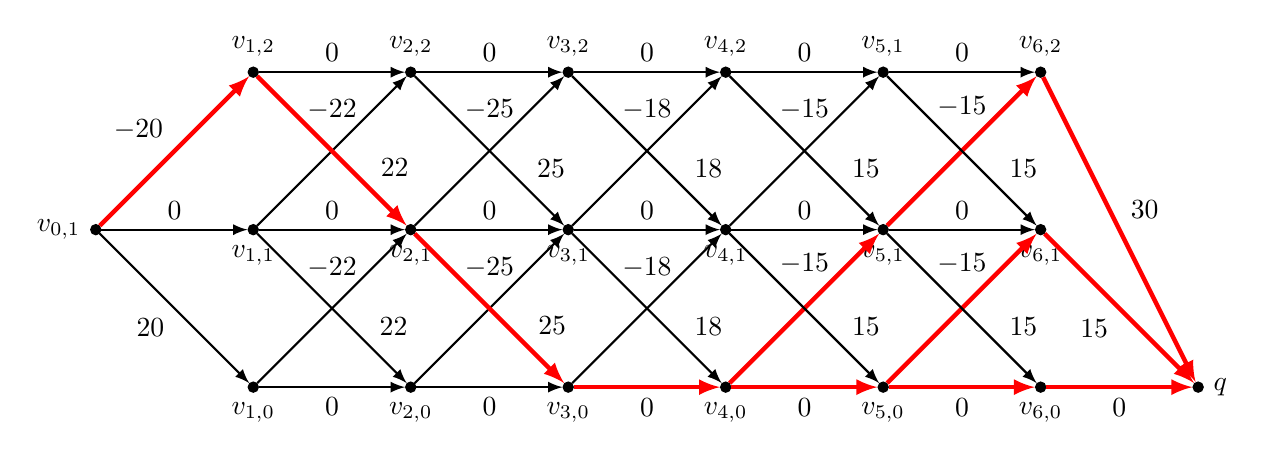
\begin{tikzpicture}

       \tikzset{enclosed/.style={draw, circle, inner sep=0pt, minimum size=.13cm, fill=black}}
%% Vertices
      	\node[enclosed, label={left: $v_{0,1}$}] (v1) at (0,2) {};
      	\node[enclosed, label={below: $v_{1,0}$}] (v2) at (2,0) {};
    		\node[enclosed, label={below: $v_{1,1}$}] (v3) at (2,2) {};
  	    \node[enclosed, label={above: $v_{1,2}$}] (v4) at (2,4) {};
     	\node[enclosed, label={below: $v_{2,0}$}] (v5) at (4,0) {};
     	\node[enclosed, label={below: $v_{2,1}$ }] (v6) at (4,2) {};
     	\node[enclosed, label={above: $v_{2,2}$}] (v7) at (4,4) {};
     	\node[enclosed, label={below:$v_{3,0}$ }] (v8) at (6,0) {};
     	\node[enclosed, label={below:$v_{3,1}$ }] (v9) at (6,2) {};
     	\node[enclosed, label={above:$v_{3,2}$ }] (v10) at (6,4) {};
     	\node[enclosed, label={below: $v_{4,0}$ }] (v11) at (8,0) {};
     	\node[enclosed, label={below:$v_{4,1}$ }] (v12) at (8,2) {};
      	\node[enclosed, label={above:$v_{4,2}$ }] (v13) at (8,4) {};
  	    \node[enclosed, label={below: $v_{5,0}$}] (v14) at (10,0) {};
  	    \node[enclosed, label={below:$v_{5,1}$ }] (v15) at (10,2) {};
     	\node[enclosed, label={above: $v_{5,1}$ }] (v16) at (10,4) {};
     	\node[enclosed, label={below:$v_{6,0}$ }] (v17) at (12,0) {};
     	 \node[enclosed, label={below:$v_{6,1}$}] (v18) at (12,2) {};
     	\node[enclosed, label={above: $v_{6,2}$}] (v19) at (12,4) {};
     	\node[enclosed, label={right: $q_{\slut}$ }] (v20) at (14,0) {};
     	
%Edges
		\path[->,>=latex,thick] (v1) edge node[midway, sloped, above, label={below, black: $20$}] {} (v2);
		\path[->,>=latex,thick] (v1) edge node[midway, sloped, below, label={above: $0$ }] {} (v3);
		\path[red,->,>=latex,ultra thick] (v1) edge node[midway, sloped, below, label={above, black: $-20$ }] {} (v4);
		\path[->,>=latex,thick] (v2) edge node[midway, sloped, above, label={below: $0$ }] {} (v5);
		\path[->,>=latex,thick] (v2) edge node[midway, above, label={above: $-22$ }] {} (v6);
		\path[->,>=latex,thick] (v3) edge node[near end, sloped, below, label={above: $22$ }] {} (v5);
		\path[->,>=latex,thick] (v3) edge node[midway, sloped, below, label={above: $0$ }] {} (v6);
		\path[->,>=latex,thick] (v3) edge node[midway, above, label={above: $-22$ }] {} (v7);
		\path[red,->,>=latex,ultra thick] (v4) edge node[near end, sloped, below, label={above, black: $22$ }] {} (v6);
		\path[->,>=latex,thick] (v4) edge node[midway, sloped, below, label={above: $0$ }] {} (v7);
		\path[->,>=latex,thick] (v5) edge node[midway, sloped, above, label={below: $0$ }] {} (v8);
		\path[->,>=latex,thick] (v5) edge node[midway, above, label={above: $-25$ }] {} (v9);
		\path[red,->,>=latex,ultra thick] (v6) edge node[near end, sloped, below, label={above,black: $25$ }] {} (v8);
		\path[->,>=latex,thick] (v6) edge node[midway, sloped, below, label={above: $0$ }] {} (v9);
		\path[->,>=latex,thick] (v6) edge node[midway, above, label={above: $-25$ }] {} (v10);
		\path[->,>=latex,thick] (v7) edge node[near end, sloped, below, label={above: $25$ }] {} (v9);
		\path[->,>=latex,thick] (v7) edge node[midway, sloped, below, label={above: $0$ }] {} (v10);
		\path[red,->,>=latex,ultra thick] (v8) edge node[midway, sloped, above, label={below,black: $0$ }] {} (v11);
		\path[->,>=latex,thick] (v8) edge node[midway, above, label={above: $-18$ }] {} (v12);
		\path[->,>=latex,thick] (v9) edge node[near end, sloped, below, label={above: $18$ }] {} (v11);
		\path[->,>=latex,thick] (v9) edge node[midway, sloped, below, label={above: $0$ }] {} (v12);
		\path[->,>=latex,thick] (v9) edge node[midway, above, label={above: $-18$ }] {} (v13);
		\path[->,>=latex,thick] (v10) edge node[near end, sloped, below, label={above: $18$ }] {} (v12);
		\path[->,>=latex,thick] (v10) edge node[midway, sloped, below, label={above: $0$ }] {} (v13);
		\path[red,->,>=latex,ultra thick] (v11) edge node[midway, sloped, above, label={below,black: $0$ }] {} (v14);
		\path[red,->,>=latex,ultra thick] (v11) edge node[midway, above, label={above,black: $-15$ }] {} (v15);
		\path[->,>=latex,thick] (v12) edge node[near end, sloped, below, label={above: $15$ }] {} (v14);
		\path[->,>=latex,thick] (v12) edge node[midway, sloped, below, label={above: $0$ }] {} (v15);
		\path[->,>=latex,thick] (v12) edge node[midway, above, label={above: $-15$ }] {} (v16);
		\path[->,>=latex,thick] (v13) edge node[near end, sloped, below, label={above: $15$ }] {} (v15);
		\path[->,>=latex,thick] (v13) edge node[midway, sloped, below, label={above: $0$ }] {} (v16);
		\path[red,->,>=latex,ultra thick] (v14) edge node[midway, sloped, above, label={below,black: $0$ }] {} (v17);
		\path[red,->,>=latex,ultra thick] (v14) edge node[midway, above, label={above,black: $-15$ }] {} (v18);
		\path[->,>=latex,thick] (v15) edge node[near end, sloped, below, label={above: $15$ }] {} (v17);
		\path[->,>=latex,thick] (v15) edge node[midway, sloped, below, label={above: $0$ }] {} (v18);
		\path[red,->,>=latex,ultra thick] (v15) edge node[midway, above, label={above,black: $-15$ }] {} (v19);
		\path[->,>=latex,thick] (v16) edge node[near end, sloped, below, label={above: $15$ }] {} (v18);
		\path[->,>=latex,thick] (v16) edge node[midway, sloped, below, label={above: $0$ }] {} (v19);
		\path[red,->,>=latex,ultra thick] (v17) edge node[midway, sloped, above, label={below,black: $0$ }] {} (v20);
		\path[red,->,>=latex,ultra thick] (v18) edge node[midway, sloped, above, label={below,black: $15$ }] {} (v20);
		\path[red,->,>=latex,ultra thick] (v19) edge node[midway, sloped, below, label={above,black: $30$ }] {} (v20);
	\end{tikzpicture}
	\caption{Længste vej igennem grafen.}
	\label{fig.gaslager_graf}
\end{figure}